
	
	\section{Когомологии групп}

	\subsection{Построение при помощи проективных резольвент}

	Пусть $G$~--- группа. Через $G$-$\Mod$ обозначим категорию модулей над $\Z[G]$. 


	Рассмотрим $\Z$, как $\Z[G]$-модуль с тривиальным действием, то есть $\forall g \in G, \ a \in \Z \ g \cdot a = a$. Построим проективную резольвенту $\Z$, как $G$-модуля. 

	Накроем $\Z$ сюръективно проективным модулем $P_0$:
	\[
		P_0 \xrightarrow{d_0} \Z \to 0.
	\]

	Теперь накроем $\Ker{d_0}$  проективным модулем $P_1$ и рассмотрим сквозное отображение $d_1\colon P_1 \to \Ker{d_1} \to P_0$. Тогда по построению $\Im{d_1} = \Ker{d_0}$, так что комплекс 
	\[
		P_1 \xrightarrow{d_1} P_0 \xrightarrow{d_0} \Z \to 0.
	\]
	будет точным в нулевом члене. Продолжая эту процедуру мы получим ацикличный комплекс из проективных модулей: 

	\[
		\ldots P_2 \xrightarrow{d_2} P_1 \xrightarrow{d_1} P_0 \overset{d_0}{\twoheadrightarrow} \Z \to 0
	\]

	Собственно он и называется \emph{проективной резольвентой} $P_{\bullet}$. 

	\begin{remark}
		Отметим, что построение выше сильно зависело от всяческих выборов. 
	\end{remark}

	Пусть теперь $P_{\bullet}$ и $Q_{\bullet}$~--- две проективные резольвенты. Построим морфизм цепных комплексов $P_{\bullet} \to Q_{\bullet}$.

	Отображение $P_0 \to Q_0$ строится просто из проективности модуля $P_0$: 

	\begin{center}
		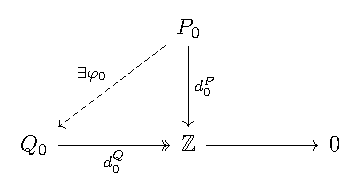
\includegraphics{lectures/6/pictures/cd_1.pdf}
	\end{center}

	Теперь заметим, что $d_0^Q  \varphi_0 d_1^P = \id_{\Z} d_0^P d_1^P = 0$, то есть $\Im{\varphi_0 d_1^{P}} \subset \Ker{d_0^Q} = \Im{d_1^Q}$. Тогда у нас есть вот такая диаграмма: 

	\begin{center}
		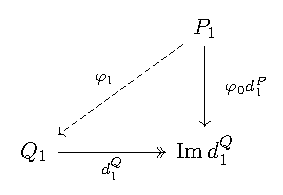
\includegraphics{lectures/6/pictures/cd_2.pdf}
	\end{center}

	Продолжая в том же духе, получаем морфизм $\varphi\colon P_{\bullet} \to Q_{\bullet}$. 

	\begin{remark}
		Отметим, что в этом рассуждении мы нигде не пользовались проективностью резольвенты $Q_{\bullet}$. Вообще говоря, только что мы доказали несколько более общее утверждение: для любого морфизма модулей $\varphi\colon M \to N$ (где $P_{\bullet}$~--- проективная резольвента $M$, а $Q_{\bullet}$~---  резольвента $N$ существует морфизм комплексов $\varphi_{\bullet} \colon P_{\bullet} \to Q_{\bullet}$ на нулевых гомологиях) совпадающий в нулевом члене с $\varphi$. У нас (здесь и далее) всегда будет $\varphi = \id$.  
	\end{remark}

	Теперь покажем, что любые два морфизма между проективными резольвентами цепно-гомотопны. Пусть $\alpha, \beta\colon P_{\bullet} \to Q_{\bullet}$~--- морфизмы цепных комлпексов, построим связывающую их цепную гопотопию $h$, то есть $h\colon P_{\bullet} \to Q_{\bullet + 1}$ такое что 
	\[
		\alpha - \beta = dh + hd.
	\]

	\begin{center}
		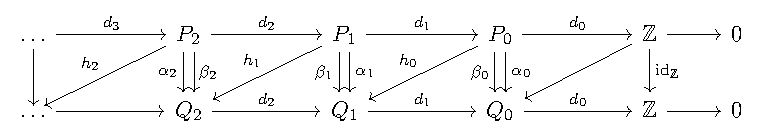
\includegraphics{lectures/6/pictures/cd_3.pdf}
	\end{center}

	Заметим, что 
	\[
		d_0^Q \alpha_0 =  d_0^Q \beta_0 \implies d_0^Q(\alpha_0 - \beta_0) = 0 \implies \Im{\alpha_0 - \beta_0} \subset \Ker{d_0^Q} = \Im{d_1^Q}.
	\]
	
	Тогда по проективности у нас есть отображение $h_0$:
	\begin{center}
		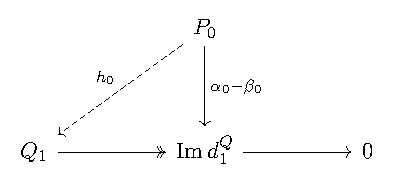
\includegraphics{lectures/6/pictures/cd_4.pdf}
	\end{center}

	Теперь построим отображение $h_1$. По построению 
	\[
		\alpha_0 - \beta_0 = h_0 d_{1}^P  \implies (\alpha_0 - \beta_0)d_1^P = d_1^Q h_0 d_1^P.
	\]
	Соотвественно, мы имеем 
	\[
		d_1^Q (\alpha_1 - \beta_1 - h_0 d_1^P) = d_1^Q(\alpha_1 - \beta_1) - (\alpha_0 - \beta_0)d_1^P = 0, 
	\]
	так как $\alpha$ и $\beta$~--- цепные отображения. Значит, $\Im{\alpha_1 - \beta_1 - h_0 d_1^P} \subset \Ker{d_1^Q} = \Im{d_2^Q}$, откуда мы снова имеем вот такую диаграмму: 
	\begin{center}
		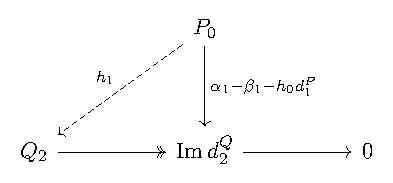
\includegraphics{lectures/6/pictures/cd_5.pdf}
	\end{center}
	и из проективности мы снова получаем отображение $h_1$. Продолжая в том же духе мы построим цепную гомотопию $h$.
 	
 	\begin{remark}
 		Таким образом, мы показали, что любые два морфизма проективных резольвент цепно-гомотопны. Итого, мы знаем, что \emph{между двумя проективными резольвентами $G$-модуля $\Z$ существует единственный с точностью до гомотопии морфизм, продолжающий $\mathrm{id}_{\Z}$}. 	
 	\end{remark}
	
	

	\begin{definition} 

		Теперь рассмотрим проективную резольвенту $P_{\bullet} \to \Z$ и применим к ней функтор $\Hom(\_, A)$, где $A \in G\text{-}\Mod$, тогда мы получим комплекс 
		\[
			 0 \to \Hom_{G}(P_0, A) \to \Hom_{G}(P_1, A) \to \Hom_{G}(P_2, A) \to \ldots
		\]

		Гомологии построенного выше комплекса 
		\[
			 0 \to \Hom_{G}(P_0, A) \xrightarrow{d_0} \Hom_{G}(P_1, A) \xrightarrow{d_1} \Hom_{G}(P_2, A) \to \ldots
		\]
		мы будем называть группами \emph{когомологий} группы $G$ с коэффициентами в $\Z[G]$-модуле $A$ и обозначать, как  $H^{i}(G, A)$. Если говорить точнее, 
		\[
			H^{i}(G, A) \eqdef Z^{i}(G, A)/B^{i}(G, A), \text{ где } Z^{i}(G, A) = \ker{d_i}, \ B^{i}(G, A) = \Im{d_{i - 1}}.
		\]
	\end{definition}

	Заметим, что пока что когомологии зависят от выбора резольвенты. Покажем, что это не так. Для этого обозначим когомологии, посчитанные при помощи одной проективной резольвенты за $H^{\bullet}(G, A)^{(P)}$, а при помощи другой за $H^{\bullet}(G, A)^{(Q)}$. 

	Тогда существует морфизм $f\colon P_{\bullet} \to Q_{\bullet}$  и $g\colon Q_{\bullet} \to P_{\bullet}$. 

	\begin{center}
		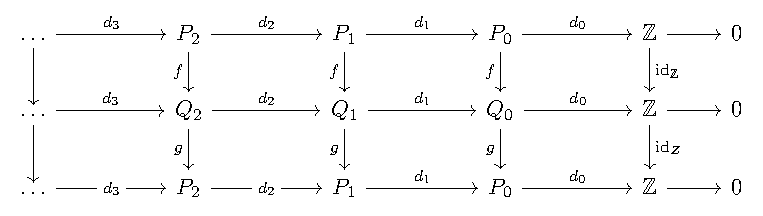
\includegraphics{lectures/6/pictures/cd_6.pdf}
	\end{center}
	Тогда, пользуясь нашим замечанием мы получаем, что $f_{*} g_{*} \sim \id$ и $g_* f_* \sim \id$. Зафиксируем гомотопию $h$ и заметим, что когда мы применим к диаграмме для неё функтор $\Hom$ у нас получится снова гомотопия, но уже для нужного комплекса. Таким образом мы получим 
	\[
		H^{q}(G, A)^{(P)} \xrightarrow{f^*} H^{q}(G, A)^{(Q)} \xrightarrow{g^*} H^{q}(G, A)^{(P)}, \text{ и } g^* f^* = \id. 
	\]
	По симметричности мы получаем, что $H^q(G, A)^{(P)} \cong H^q(G, A)^{(Q)}$.

	Как и всегда, стандартным образом из которткой точной последовательности коэффициентов получается длинная точная последовательность когомологий: 

	\begin{theorem}[Длинная точная последовательность когомологий] 
		Пусть $0 \to A \to B \to C$~--- точная последовательность $G$-модулей. Тогда имеется естественная длинная точная последовательность групп когомологий:
		\begin{multline*}
			0 \to H^{0}(G; A) \to H^{0}(G; B) \to H^{0}(G; C) \to H^{1}(G; A) \to H^{1}(G; B) \to \ldots \to \\ \to H^{n}(G; A) \to H^{n}(G; B) \to H^{n}(G; C) \to H^{n + 1}(G, A) \to \ldots
		\end{multline*}
	\end{theorem}

	\subsection{Стандартная резольвента}

	Как мы видели в предыдущем параграфе, когомологии группы $G$ с коэффициентами в $G$-модуле $A$ не зависят от выбора проективной резольвенты. В данном параграфе мы приведём \emph{стандартную резльвенту}, которая часто оказывается весьма удобной при вычислениях. ъ

	\begin{definition} 
		\emph{Стандратная проективная резольвента } для $\Z$~--- это свободная резольвента 
		\[
			\ldots \Z[G^{i}] \to \Z[G^{i + 1}] \to \ldots \to \Z[G^2] \to \Z[G] \xrightarrow{\varepsilon} \Z \to 0.
		\]
		Напомним, что $P_i = \Z[G^{i + 1}]$~--- свободный $\Z[G]$-модуль с базисом $G \times G \times \ldots \times G$ (где произведение берётся $i + 1$ раз). Группа $G$ действует на каждый базисный элементы естественным образом: 
		\[
		 	s \cdot (g_0, \ldots, g_i) = (s g_0, \ldots, s g_i).
		 \] 
		 Гомоморфизм $d\colon \Z[G^i] \to \Z[G^{i - 1}]$ определяется стандартным образом: 
		 \[
		 	d_i(g_0, \ldots, g_i) = \sum_{j = 0}^{i} (-1)^j (g_0, \ldots, g_{j - 1}, g_{j + 1}, \ldots, g_{i}). 
		 \]
 	\end{definition}

 	Заметим, что тогда 
 	\[
 		\Hom_{G}(\Z[G^{i + 1}], A) = \{ f \colon G^{i + 1} \to A \ \vert \  f(\sigma g_0, \ldots, \sigma g_i) = \sigma g(g_0, \ldots, g_i) \}. 
 	\]
 	Заметим, что такая функция полностью определяется своими значениями на элементах из $G^{i + 1}$ вида $(1, g_1, g_1 g_2, \ldots, g_1 g_2 \ldots g_i)$. Соответственно, если мы обозначим 
 	\[
 		\varphi(g_1, \ldots, g_i) = f(1, g_1, g_1 g_2, \ldots, g_1 \ldots g_i),
 	\]
 	то дифференциал в комплексе $\Hom_{G}(\Z[G^{\bullet}], A)$ можно записать в таком виде: 
 	\[
 		(d\varphi)(g_1, \ldots, g_{i + 1}) = g_1 \dot \varphi(g_2, \ldots, g_{i + 1}) + \sum_{j = 1}^i (-1)^j \varphi(g_1, \ldots, g_{j} g_{j + 1}, \ldots, g_{i + 1}) + (-1)^{i + 1} \varphi(g_1, \ldots, g_i). 
 	\]

 	Найдём теперь конструктивное описание некоторых групп когомологий. 

 	\begin{example}[Нулевая группа когомологий]
 		По определению $H^{0}(G, A) \cong \ker{d_1}$. Теперь заметим, что из точности последовательности 
 		\[
 			P_1 \to P_0 \to \Z \to 0
 		\]
 		следует точность последовательности 
 		\[
 			0 \to \Hom_{G}(\Z, A) \xrightarrow{\varphi} \Hom_{G}(P_0, A) \xrightarrow{d_0} \Hom_{G}(P_1, A),
 		\]
 		откуда $\ker{d_0} = \Im{\varphi}$, а так как $\varphi$~--- мономорфизм, $\Im{\varphi} \cong \Hom_{G}(\Z, A)$. Таким образом, 
 		\[
 			H^{0}(G, A) \cong \Hom_{G}(\Z, A).
 		\]
 		Также отметим, что $\Hom_{G}(\Z, A) \cong A^{G}$, где $A^G = \{ a \in A \ \vert \ ga = a \ \forall g \in G \}$~--- неподвижные точки. Второй изоморфизм строится так: 
 		\[
 			\Hom_{G}(\Z, A) \ni \varphi  \mapsto \varphi(1).
 		\]
 		Сначала заметим, что он вообще действует в $A^{G}$, так как $\forall n \in \Z \ \varphi(gn) = g\varphi(n)$ с одной стороны, а с другой, так как $\Z$ у нас действует на $G$ тривиально, $\varphi(gn) = \varphi(n)$, т.е. $\varphi(n) = g \varphi(n) \ \forall n \in \Z$.

 		Очевидно, что этот гомоморфизм инъектвен, покажем, что он сюръективен. Действительно, для $a \in A^G$ положим $\varphi(1) = a$, а далее доопределим $\varphi$ по линейности и $G$-эквивариантности (т.е. положим $\varphi(n) = na$). Таким образом, 
 		\[
 		 	H^{0}(G, A) \cong A^{G}.
 		 \] 
 		
 	\end{example}

 	\begin{example}[Первая группа когомологий]
 		При помощи явной формулы для дифференцицала мы сразу видим, что 
 		\[
 			Z^{1}(G, A) = \ker{d_2} = \{ \varphi\colon G \to A \ \vert \ \varphi(g_1 g_2) = g_1 \varphi(g_2) + \varphi(g_1)\}.
 		\]
 		Т.е. коциклами являются \emph{скрещенные гомоморфизмы}, т.е. отображения $\varphi\colon G \to A$, для которых выполнено тождество $\varphi(g_1 g_2) = g_1 \varphi(g_2) + \varphi(g_1)$. Кроме того, сразу видно, что 
 		\[
 			B^{1}(G, A) = \Im{d_1} =  \{ \varphi \colon G \to A \ \vert \ \exists a \in A \colon \varphi(g) = ga - a \}. 
 		\]
 		Соответственно, мы имеем $H^{1}(G, A) = Z^{1}(G, A) / B^{1}(G, A)$. Приведём теперь несколько примеров.

 		Пусть $A = \Z$ с тривиальным действием. Тогда $\varphi(g_1 g_2) = g_1 \varphi(g_2) + \varphi(g_1) = \varphi(g_2) + \varphi(g_1)$, и 
 			\[
 				Z^{1}(G, \Z) = \Hom_{\Grp}(G, \Z). 
 			\]
		 Кроме того, так как $ga - a = a - a = 0$, мы имеем $B^{1}(G, \Z) = 0$. Таким образом,
		 \[
		 	H^{1}(G, \Z) \cong \Hom_{\Grp}(G, \Z).
		 \]

		 \begin{itemize}
		 	\item Пусть теперь $G$~--- конечная группа. Тогда $\forall g \ \exists n \colon g^n = e$. Тогда $\varphi(g^n) = n \varphi(g) = \varphi(e) = 0$, откуда $\varphi(g) = 0$. Таким образом, $\Hom_{\Grp}(G, \Z) = 0$. 

		 	\item Если же $G = \Z$, то 
		 	\[
		 		\Hom_{\Grp}(\Z, \Z) \cong \Z \implies H^1(\Z, \Z) \cong \Z.
		 	\]
		 \end{itemize}

 	\end{example}
	
	\begin{definition} 
		Пусть $A, B \in G\text{-}\Mod$. Тогда на $\Hom(A, B)$ можно завести структуру $G$-модуля следующим образом: пусть $\varphi \in \Hom(A, B)$, тогда определим 
		\[
			g\varphi\colon A \to B, \quad g\varphi(a) = g \cdot \varphi(g^{-1}a). 
		\]
	\end{definition}

	\begin{remark}
		Также заметим, что $\Hom(A, B)^{G} = \{ \varphi \in \Hom(A, B) \ \vert \ \forall g \in G g \varphi = \varphi \} $, но в то же время 
		\[
			g\varphi = \varphi \Leftrightarrow g \varphi(g^{-1}a) = \varphi(a) \Leftrightarrow \varphi(g^{-1} a) = g^{-1}\varphi(a),
		\]
		откуда видно, что $\Hom(A, B)^{G} = \Hom_{G}(A, B)$. 
		
	\end{remark}

	\begin{definition} 
		Пусть $X$~--- абелева группа с тривиальным действием  $G$.  Тогда модуль вида $\Hom(\Z[G], X)$ мы будем называть \emph{коиндуцированным}. 
	\end{definition}

    Заметим, что есл $A = \Hom(\Z[G], X)$~--- коиндуцированный модуль, то для любого $B \in G\text{-}\Mod$
	\[
		\Hom_{G}(B, A) \cong \Hom_{G}(B, X) \Leftrightarrow \Hom_{G}(B, \Hom(\Z[G], X)) \cong \Hom_{G}(B, X).
	\]
	Действительно, изоморфизм строится таким образом: 
	\[
		\varphi\colon B \to A, \ \varphi \mapsto \psi\colon B \to X, \ \psi(b) = \varphi(b) \cdot 1. 
	\]
	Обратное же отображение стротся так: 
	\[
		f \in \Hom_{G}(B, X), \ f \mapsto \varphi\colon b \mapsto s_b \text{ где } s_b(\sigma) = f(\sigma^{-1}b).
	\]
	Легко видеть, что эти отображения взаимнообратны. Теперь мы видим, что наш комплекс (который вычисляет когомологии) приобретает вот такой вид: 
	\begin{center}
		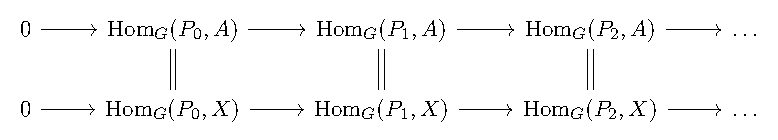
\includegraphics{lectures/6/pictures/cd_21.pdf}
	\end{center}

	Заметим, что проективные модули свободны как абелевы группы (так как являются прямыми слагаемыми свободных), а на них функтор $\Hom_{G}(\_, X)$ точен. Соответственно, полученный комплекс будет точен в каждом члене, начиная со второго. Соответственно, мы получили, что если $A$~--- коиндуцированный модуль, то 
	\[
		H^{q}(G, A) = 0 \quad \forall q \ge 1.
	\]
	

	Теперь пусть $A$~--- произвольный $G$-модуль, тогда мы можем рассмотреть $A^* = \Hom(\Z[G], A)$. Тогда существует естественное вложение $A \hookrightarrow A^*$ по правилу $a \mapsto \varphi_a$, где $\varphi_a(g) = g^{-1}a$. Соответственно, у нас есть короткая точная последовательность модулей  
	\[
		0 \to A \to A^* \to A' \to 0,
	\]
	где $A' = A^*/A$. Если мы напишем длинную точную последовательность когомологий, то, так как $H^{q}(G, A^*) = 0 \quad \forall q \ge 1$, свзывающий гомоморфизм даст нам изоморфизмы 
	\[
		\delta \colon H^{q}(G, A') \xrightarrow{\sim} H^{q + 1}(G, A),
	\]
	что часто позволяет вести индукцию по размерности. 





 
 

	
 





